\chapter{\MakeUppercase{État de l'art sur les images radar à ouverture synthétique}}
% TODO: 
\section{Introduction}

\section{Remote sensing}

\section{Images radar à ouverture synthétique}
L'imagerie par Radar à Ouverture Synthétique (Synthetic Aperture Radar, SAR) est une technique de télédétection permettant d'obtenir des images de haute résolution indépendamment des conditions d'éclairage et, dans une large mesure, des conditions météorologiques \cite{ramkumar_survey_2020}. Des ondes radio ont été utilisé pour obtenir ces images. Contrairement à l'imagerie optique qui repose sur la lumière visible, les systèmes SAR  exploitent des ondes radio bien plus longues, généralement comprises entre 3 cm et quelques mètres. Comme l'illustre la \Cref{fig-chap1:spectre_electromagnetique} ci-dessous, ces longueurs d'onde appartiennent à la bande des micro-ondes du spectre électromagnétique.
\begin{figure}[H]
    \centering
    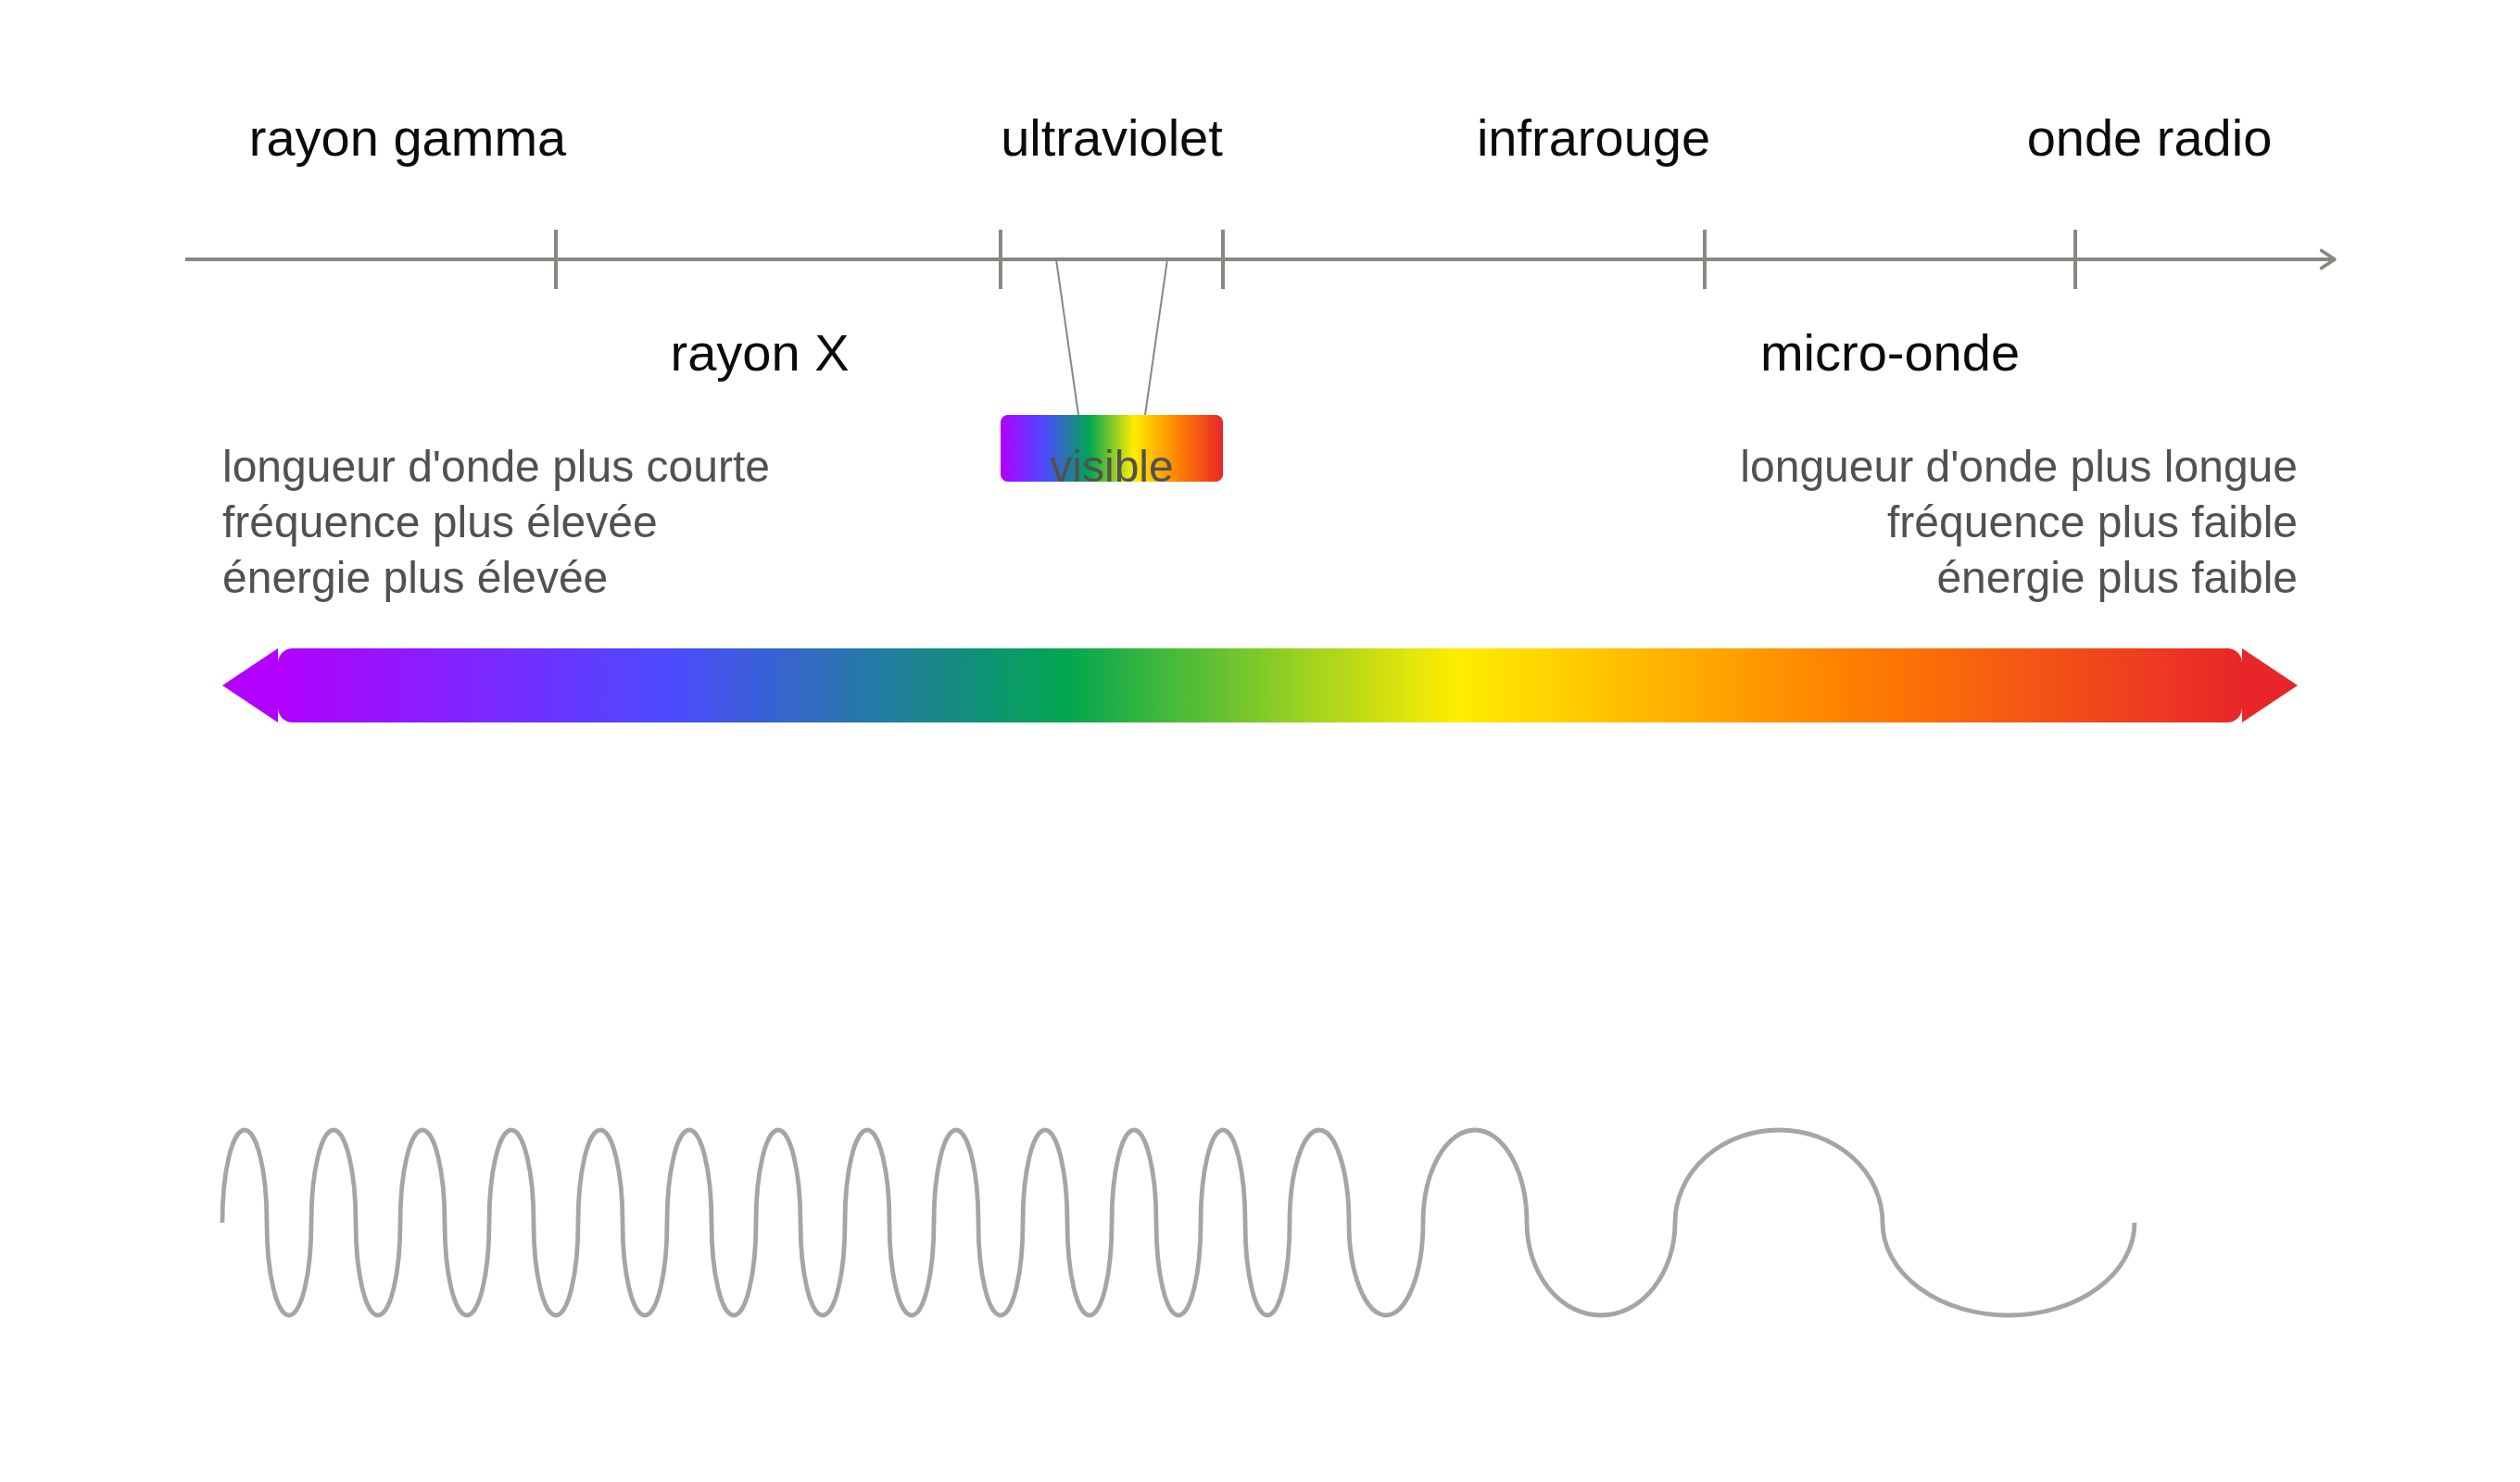
\includegraphics[height=10cm, keepaspectratio]{images/chap1/spectre_electromagnetique.png}
    \caption{Comparaison de la longueur d'onde, de la fréquence et de l'énergie dans le spectre électromagnétique}
    \label{fig-chap1:spectre_electromagnetique}
\end{figure}

Un radar SAR émet ses propres ondes électromagnétiques et enregistre les échos réfléchis par les objets observés, ce qui lui permet de fonctionner aussi bien de jour que de nuit, ainsi qu'à travers les nuages, la pluie ou le brouillard.

\subsection{Concepts fondamentaux}
Dans un radar à ouverture réelle (Real Aperture Radar, RAR), la résolution en azimut (ou résolution transversale) dépend directement de la longueur physique de l'antenne, de la longueur d'onde du signal radar et de la distance entre le capteur et la cible. Elle est donnée approximativement par :

\begin{equation}
    \Delta_{az} \approx \cfrac{\lambda \mathrm{R}}{\mathrm{D}}
\end{equation}
où \(\lambda\) est la longueur d'onde, \(\mathrm{R}\) la distance entre le radar et la cible, et \(\mathrm{D}\) la longueur de l'antenne.
Donc, plus l'antenne est petite, moins l'image est nette et cet effet s'aggrave avec la distance.
Concrètement, pour avoir une image nette depuis un satellite, par exemple, à des centaines de kilomètres d'altitude, il faudrait une antenne physique de plusieurs kilomètres de long. Évidemment, impossible à construire ou à faire voler.\\
Le principe du radar à ouverture synthétique consiste à contourner cette limitation en exploitant le déplacement de la plateforme porteuse (satellite, avion ou drone). Au lieu d'utiliser une antenne physique de très grande dimension, le système acquiert les échos radar depuis une succession de positions le long de la trajectoire de vol. Grâce à la connaissance précise de la géométrie d'acquisition et à un traitement numérique cohérent des signaux, ces mesures sont combinées pour simuler une antenne beaucoup plus longue que l'antenne réelle. Cette antenne virtuelle est appelée ouverture synthétique.
\subsection{Formation des images SAR}
\subsection{Caractéristiques des images SAR}